\chapter{Beispiele für Digital Nudges}
\section{IKEA: Positives Vorbild im E-Commerce}
\subsection{Einführung in das Beispiel und Problemstellung}
Vor allem im Bereich Wohnen ist Kunden eine große Auswahl wichtig. Es erlaubt sowohl Individualisierung bei der Gestaltung eines Wohnraumes, als auch Anpassung an das vorhandene Budget. Dadurch wird die Zielgruppe vergrößert und mehr Umsatz generiert. Bei einer zu großen Auswahl an Optionen wird häufig ein umgekehrtes Phänomen beobachtet, dem Choice Overload Effect, zu Deutsch das Auswahlparadoxon. \parencite[S. 58]{Bauer.2018}

Dieses beschreibt die Tendenz von Kaufenden, eine große Auswahl zu favorisieren, zu einer Kaufentscheidung kommt es allerdings häufiger, wenn weniger Optionen zur Verfügung stehen. Das liegt daran, dass potenzielle Kunden den Überblick verlieren und sich überfordert fühlen. \parencite[S. 58]{Bauer.2018}Die Konsequenz ist oft die Aufschiebung der Entscheidung, der Wechsel zur Konkurrenz mit weniger Auswahl. Eine andere Möglichkeit, vor allem im digitalen Umfeld, ist die spontane Entscheidung für ein Produkt. Erst nach dem Kauf werden die Details näher betrachtet, und möglicherweise festgestellt, dass das Produkt nicht den Wünschen und Anforderungen entspricht.

Vor diesem Problem steht auch die Firma IKEA. Laut ihrer Website gibt es allein für die Kategorie Betten 2410 Modelle mit verschiedenen Ausführungen

und Kombinationen.\parencite{InterIKEASystemsB.V..2022} Dieses Produktportfolio ist wichtig für IKEA, um mit den verschiedenen Preiskategorien und Designlinien möglichst viele Kunden anzusprechen. Allerdings sind selbst nach der Auswahl von Filtern noch bis zu hundert verschiedene Optionen verfügbar. Diese unterscheiden sich meist nur in kleinen Details. Um den Kunden den Vergleich ihrer Auswahl zu vereinfachen, setzt IKEA Digital Nudging ein.
\subsection{Aufbau und Wirkung}
\begin{figure}[ht]
    \centering
    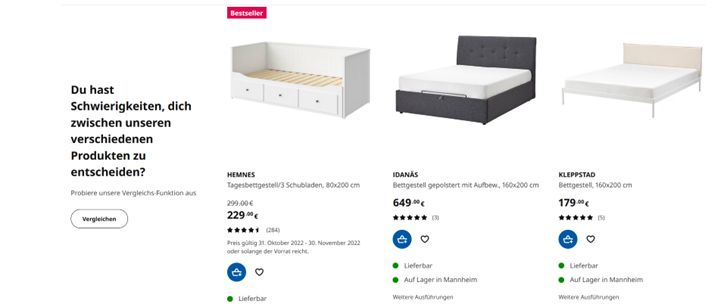
\includegraphics[width=0.9\textwidth]{Bilder/Ikea_Nudge.png}
    \caption{Nudge zum Nutzen der Vergleichsfunktion auf \url{https://www.ikea.de} in der Produktsuche}
    \label{fig:Ikea-Nudge}
\end{figure}
In der zweiten Reihe der angezeigten Optionen nutzt IKEA die linke Spalte, um den Nutzenden auf die Vergleichen-Funktion hinzuweisen. Der Hinweis ist so angebracht, dass er für Nutzende, die das vorhandene Angebot überfliegen möchten, nicht störend ist. Dennoch ist er auffällig genug, um wahrgenommen zu werden. Im Fokus steht vor allem der deutlich größere Schriftzug, welcher die Probleme des Nutzenden anspricht. Direkt darunter wird die Vergleichen-Funktion als Lösung aufgezeigt.

\subsection{Bewertung anhand der ethischen Grundlagen}
Der Nudge ermöglicht Nutzenden die freie Entschidung, ob die Vergleichen-Funktion genutzt wird. Es wird auch nicht aktiv von der Website versucht, den User zur Verwendung der Funktion zu überzeugen. Der Nudge ermöglicht dem Kaufenden eine bessere Entscheidung bezogen auf den Kauf des Produktes. Dadurch bleibt die Autonomität des Nutzenden bestehen, und wird bei der Kaufentscheidung zusätzlich verstärkt.

Auch sind die Auswahlfelder klar erkennbar, und verleiten den User nicht dazu, Optionen auszuwählen die er nicht versteht bzw. nicht auswählen wollte. Die Benennung ist klar verständlich und nicht umzudeuten. Hinter dem Button sind auch nicht zusätzliche Funktionen oder Aktionen versteckt, die der Nutzende eigentlich nicht auswählen wollte. Auch verzichtet IKEA auf Voreinstellungen und erlaubt es dem User seine Suche individuell anzupassen. Diese Punkte sprechen für eine hohe Transparenz des Nudges, was die zweite ethische Grundlage erfüllt.

Bei der Zielrechtfertigung ist IKEA darauf fokussiert, die User Experience für interessierte Personen zu verbessern, und diese dadurch eher zum Kauf zu bewegen. Das bringt zwar positive Aspekte für IKEA, jedoch ist das Hauptziel des Nudges, den Besuch der Website für Kunden möglichst angenehm zu gestalten.

\section{Cookie Banner: Manipulativ?}
\subsection{Einführung in das Beispiel und Problemstellung}
Internetseiten nutzen zum Anzeigen und Senden von Daten das sogenannte \ac{HTTP}. Bei \ac{HTTP} handelt es sich um ein sogenanntes ``stateless'' (zustandsloses) Protokoll, d.h. alle Anfragen und Transaktionen zwischen dem Nutzer und der aufgerufenen Internetseite sind unabhängig voneinander. Dadurch fällt es schwer, Zusammenhänge und Nutzerdaten mehrerer Anfragen mitzusenden und abrufbar zu halten.

Cookies werden eingesetzt, wenn bestimmte Infos zwischen mehreren Anfragen gespeichert werden sollen. Sie sind kleine Dateien, welche von der aufzurufenden Internetseite angefordert und gesendet werden. Die Cookies werden dann vom genutzten Internetbrowser angelegt und verwaltet. Sie sind dabei immer spezisich für die Seite, die sie anfragt und sendet und werden genutzt, um beispielsweise Internetseiten mit Kontofunktionen zu realisieren. \parencite[S. 4-6]{Kristol.}

Obwohl Cookies spezifisch für jede Internetseite sind und ein Verknüpfen von Nutzerdaten über mehrere Internetseiten hinweg nicht möglich sein sollte, wurde durch die Funktionsweise des Internets schnell eine Möglichkeit gefunden, Cookies für mehrere Seiten zu nutzen.

Dabei wird neben der gewünschten Internetseite noch eine weitere Seite geladen, welche den Cookie setzt und anfordert. Wenn dieses System über mehrere Internetseiten hinweg genutzt wird, können die Interessen eines Nutzers nachverfolgt werden. Man spricht hierbei vom ``Third Party Cookies'', da das Datensammeln nicht direkt durch den Seitenbetreiber selbst passiert. \parencite[S. 2608]{Bielova.2017}

\begin{figure}[ht]
	\centering
	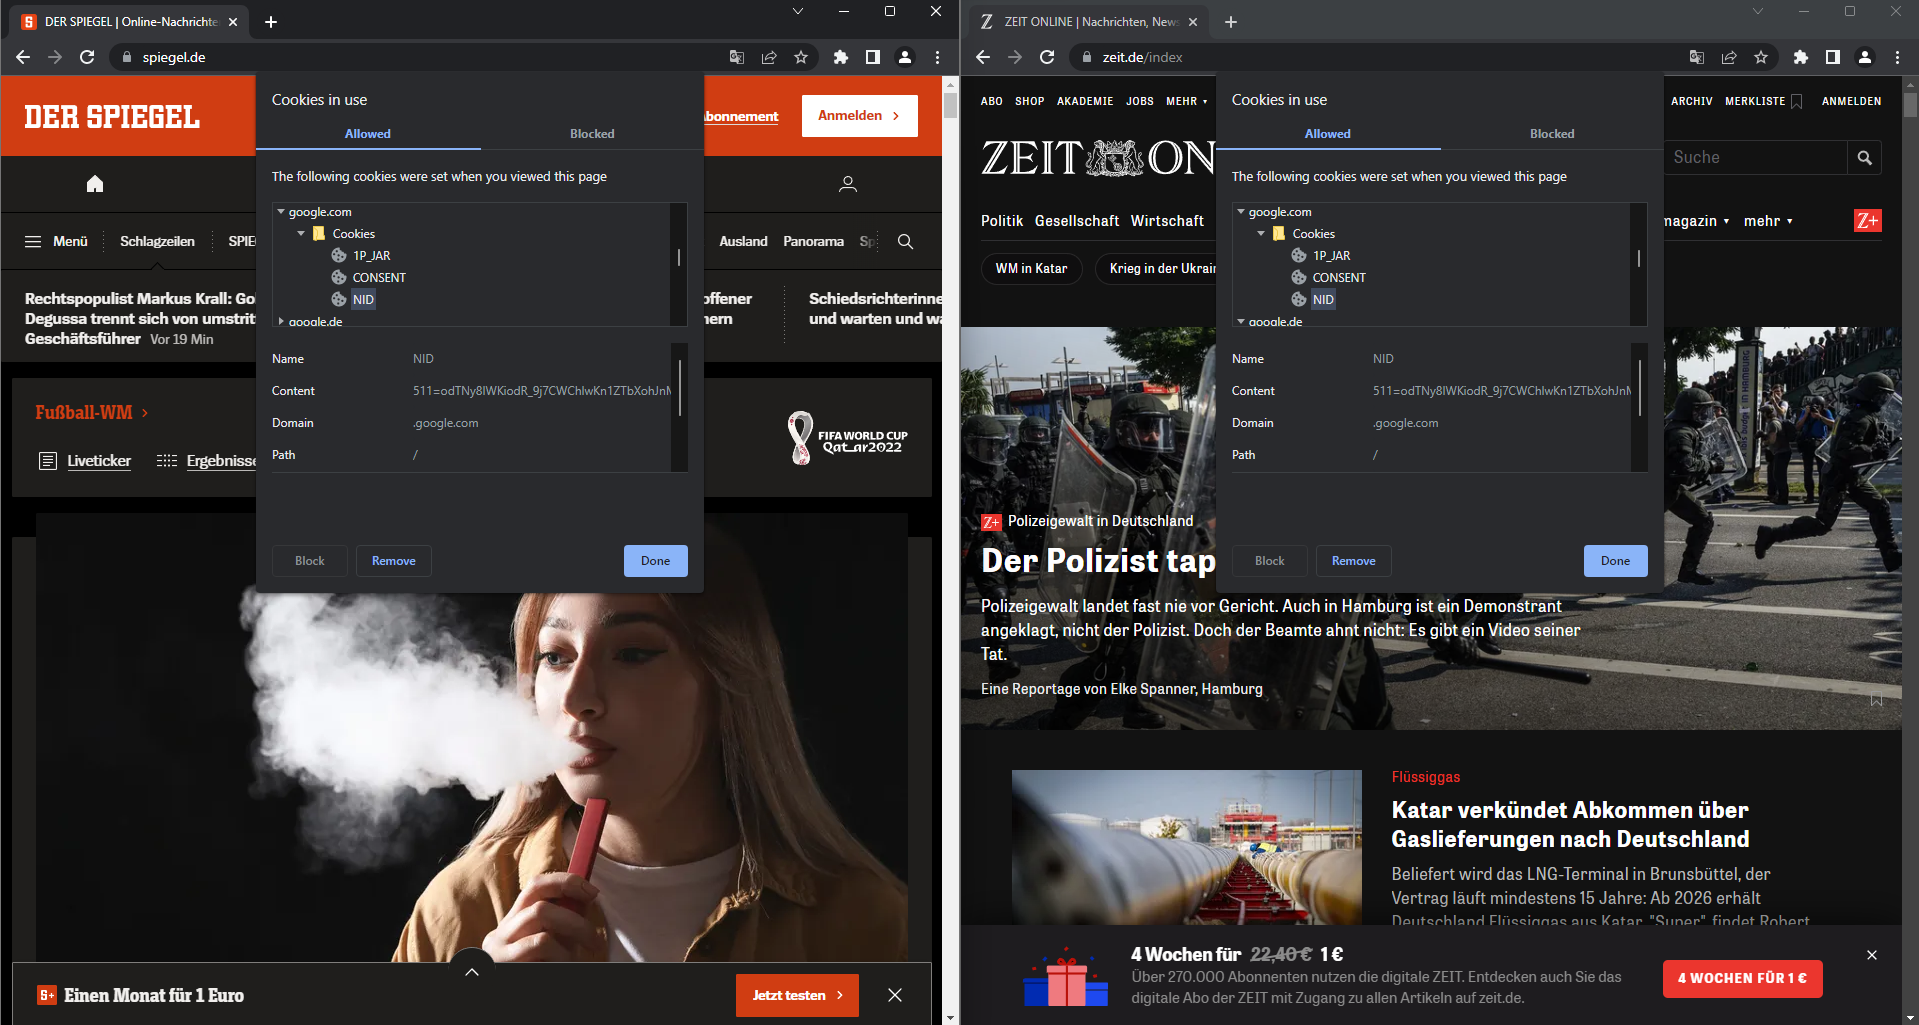
\includegraphics[width=1\textwidth]{Bilder/Cookies.png} 
	\caption{Ein Third Party Cookie von Google, welcher bei \url{https://www.spiegel.de} und \url{https://www.zeit.de} genutzt wird}
	\label{fig:Third-Party}
\end{figure}

Die \ac{EU} hat 2016 die \ac{DSGVO} verabschiedet. \parencite{EuropaischeUnion.2016} Seitdem gibt es für Cookies in der \ac{EU} einen rechtlichen Rahmen zur Verwendung jener. Dieser sieht vor, dass lediglich ``First Party Cookies'', also Cookies, welche direkt von der aufgerufenen Internetseite erstellt werden, genutzt werden dürfen. Entsprechenden ``Third Party Cookies'', welche hauptsächlich zum Sammeln von Nutzerdaten genutzt werden, muss der Nutzer nach der \ac{DSGVO} erst explizit zustimmen. Die \ac{EU} erhofft sich davon mehr Transparenz im Bezug auf die Verarbeitung personenbezogener Daten. \parencite[S. 84]{EuropaischeUnion.2016}

Unternehmen ist in vielen Fällen jedoch daran gelegen, möglichst viele ``Third Party Cookies'' einzubinden. So gibt es ganze Geschäftsmodelle, welche Cookies zu Werbe- und Analysezwecken nutzen und durch das effektive Sammeln und Auswerten von Daten Umsatz generieren.\parencite[S. 418-420]{.2012} Durch die gegebenen Umstände entwickelte sich so der Trend, dass zur Einwilligung in die Datensammlung ein Nudge genutzt wird, welcher die Entscheidung beeinflussen soll.

\subsection{Aufbau und Wirkung}
Die Zustimmung zu Cookies wird auf Internetseiten meist in Form eines Banners realisiert, welcher den Nudge enthält. Der Cookie Banner fragt dabei den Nutzer, ob das Einsetzen von Drittanbieter Cookies und damit das Sammeln von Daten gestattet ist. Die Gestaltung weicht dabei je nach Plattform stark voneinander ab.

\begin{figure}[ht]
    \centering
    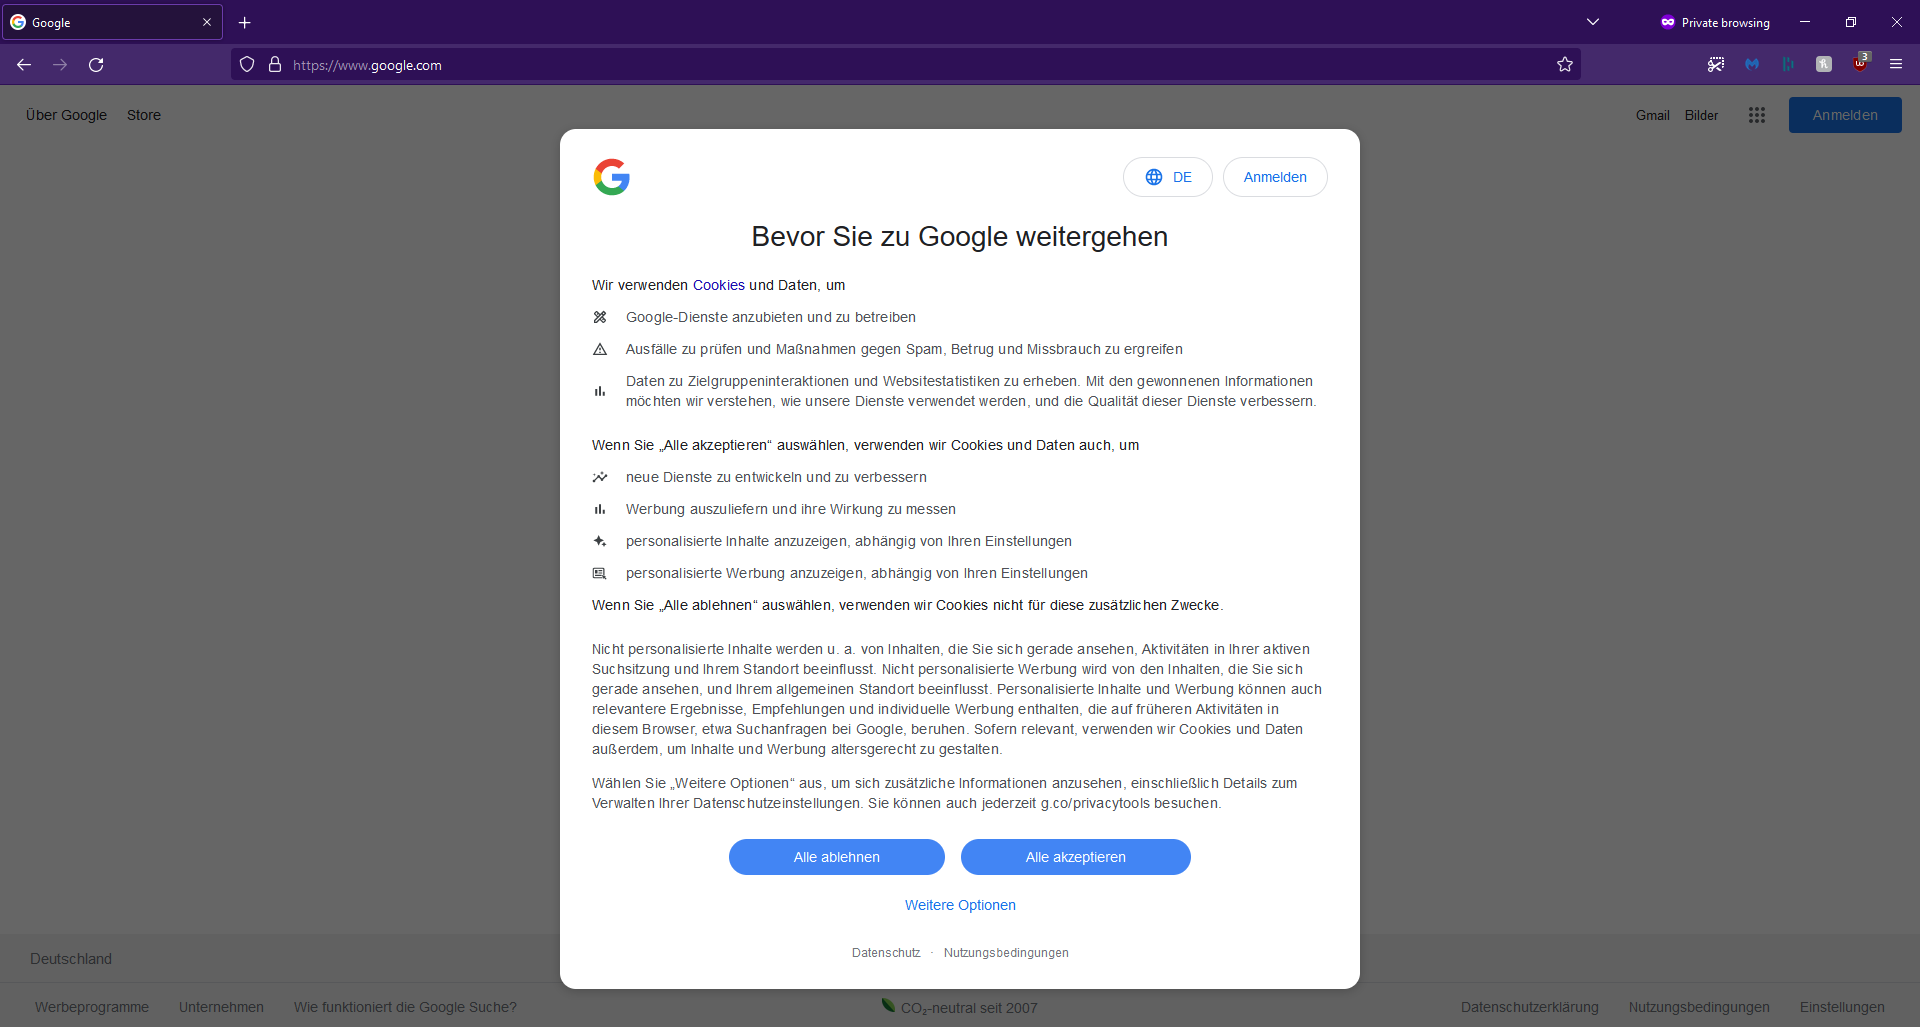
\includegraphics[width=1\textwidth]{Bilder/Google_Banner.png}
    \caption{Cookie Banner auf \url{https://www.google.com}}
    \label{fig:Google-Cookie}
\end{figure}

Beim ersten Aufrufen der Website \url{https://www.google.com} wird der Cookiebanner angezeigt. Dabei wird bereits direkt ein Nudge auffällig. Der Banner wird zentral über dem eigentlichen Inhalt des Bildschirms platziert. Der Nutzer, welcher gerade etwas bei Google suchen möchte, muss daher zuerst mit dem Banner interagieren. Google bietet hier einen Knopf ``Alles Akzeptieren'' und ``Alles ablehnen'' an. Dennoch wird hier bereits Einfluss auf den Nutzer genommen, da sein Nutzungserlebnis direkt gestört wird und er erst einen der beiden Knöpfe drücken muss, um mit seiner Arbeit fortzufahren.

Auf der Webseite von Facebook (\url{https://www.facebook.com/de}) wird neben dem inhaltsverdeckenden Banner ein weiterer Nudge eingesetzt. Die Option ``Erforderliche und optionale Cookies erlauben'' ist in einem auffälligen Blau markiert, während die Option ``Nur erforderliche Cookies erlauben'' in einer grauen Farbe gezeigt wird.

\begin{figure}[ht]
    \centering
    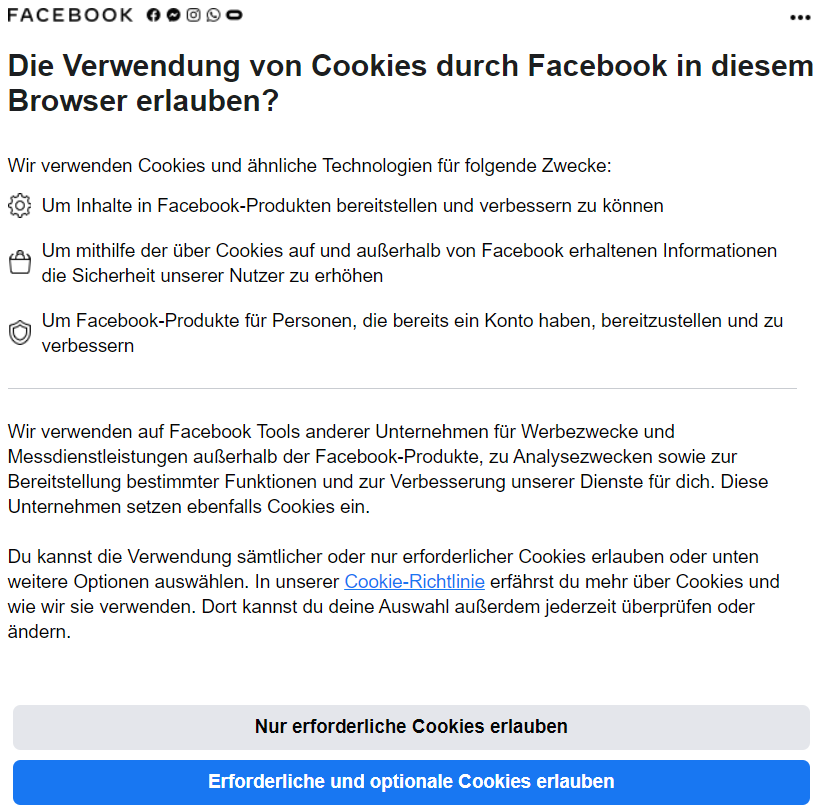
\includegraphics[width=0.8\textwidth]{Bilder/Facebook_Banner.png}
    \caption{Cookie Banner auf \url{https://www.facebook.com/de} mit farblich unterschiedlichen Knöpfen}
    \label{fig:Facebook-Cookie}
\end{figure}

Die farbliche Hervorhebung einer Option erscheint für den Nutzer hierbei wie eine Empfehlung und sticht mehr ins Auge, als der hellgraue Farbton, welcher sehr ähnlich zum Hintergrund wirkt. Hervorhebung einer gewünschten Option kann nicht nur durch Farbe, sondern auch durch Positionierung und Größe innerhalb des Banners passieren.

Eine weitere Möglichkeit, den Nutzer in seiner Entscheidung zu beeinflussen, stellt das Verlagern der Ablehnen Funktion auf eine Extra Seite dar. Hierbei wird dem Nutzer lediglich eine Option zum Akzeptieren und eine Option zum Ansehen diverser Einstellungen bezüglich des Datenschutzes angeboten.

\begin{figure}[ht]
    \centering
    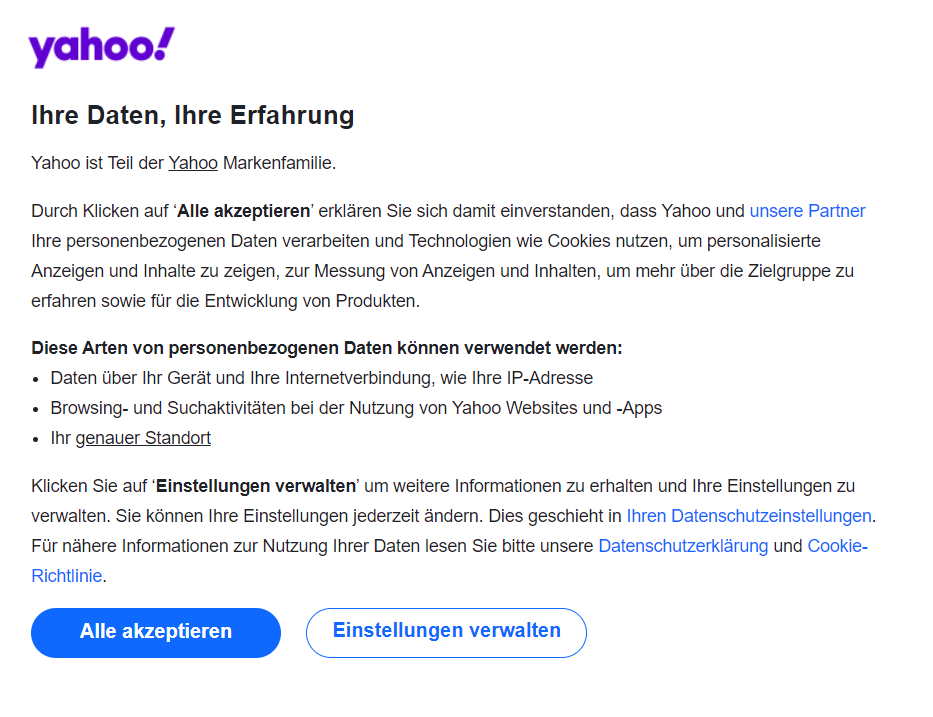
\includegraphics[width=0.8\textwidth]{Bilder/Yahoo_Banner.png}
    \caption{Cookie Banner auf \url{https://www.yahoo.de} mit Einstellungsknopf}
    \label{fig:Yahoo-Cookie}
\end{figure}

Dieses Verlagern der Ablehnenfunktion auf eine weitere Seite ist besonders effektiv, wenn der Nudge dazu genutzt werden soll, dass Nutzer tendenziell dem Datensammeln zustimmen. Die Zustimmung aller Cookies ist 22 - 23 \% wahrscheinlicher, wenn die Ablehnenfunktion nicht direkt im Banner enthalten ist. \parencite[S. 8]{Nouwens.2020}

\subsection{Bewertung anhand der ethischen Grundlagen}

Je nach Funktionsweise lässt sich nachweisen, dass die hier gezeigten Beispiele gegen die in Kapitel HIER EINSETZEN verstoßen.
Während die Einblendung von Google (siehe Abbildung \ref{fig:Google-Cookie}) mit den Optionen ``Alles Akzeptieren'' und ``Alles ablehnen'' eine transparente und autonome Auswahl der Einstellungen ermöglicht, lässt sich argumentieren, dass die Banner von Facebook (siehe Abbildung \ref{fig:Facebook-Cookie}) und Yahoo (siehe \ref{fig:Yahoo-Cookie}) gegen ethische Grundsätze von digitalen Nudges verstoßen.

In beiden Fällen ist die Transparenz eingeschränkt, da eine Option (Alles akzeptieren) farblich hervorgehoben ist und die Wahl damit nicht mehr neutral ist. Yahoo geht außerdem einen Schritt weiter und bietet gar nicht mehr alle Optionen direkt an (``Alles ablehnen''), sondern versteckt den Inhalt auf einer Einstellungsseite, was nicht nur Transparenz sondern auch Autonomie einschränkt.

Deutsche Zeitungsanbieter nutzen dieses Prinzip und bieten keine Option zum Ablehnen mehr an. Hier wird lediglich vorgeschlagen, die Cookierichtlinien zu akzeptieren oder für ein cookiefreies Modell zu bezahlen.

\begin{figure}
    \centering
    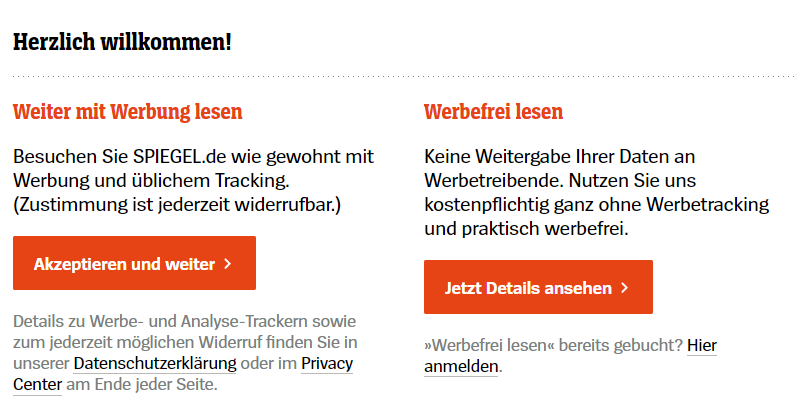
\includegraphics[width=0.9\textwidth]{Bilder/Spiegel_Banner.png}
    \caption{Cookie Banner auf \url{https://www.spiegel.de} mit Bezahlfunktion}
    \label{fig:Spiegel-Cookie}
\end{figure}

Hier sind Autonomität und Transparenz noch eingeschränkter, da gar nicht mehr alle Optionen (Cookies ablehnen) angeboten werden. Dem Nutzer wird lediglich angeboten, alle Cookies zu akzeptieren, eine Option alles abzulehnen gibt es nicht mehr.

Abschließend lässt sich sagen, dass die Nutzung von Cookie Bannern bei bekannten Plattformen klar gegen ethische Grundlagen verstößt. Neben den Idealen der Autonomität und Transparenz, verstoßen alle genannten Beispiele auch gegen den Grundsatz der Zielrechtfertigung, da mit dem Aktivieren der Cookies weder soziale noch nutzerfreundliche und lediglich Interessen der Plattform verfolgt werden. Auch rechtlich sind die gezeigten Beispiele bereits kritisiert worden. So verurteilte die französische Datenschutzbehörde Facebook und Google zu hohen Geldstrafen aufgrund von Verstößen gegen die DSGVO im Bezug auf die Implementierung von Cookie-Bannern. \parencite{AnnaBiselli.2022}